\subsubsection{ERD tổng thể}
% ------------------- MÔ TẢ DATABASE ------------------------------------
\paragraph{Dữ liệu về thành viên}

\begin{itemize}[leftmargin=*]
    \item \textbf{USER}: Thông tin chung
    \begin{itemize}
        \item Họ tên (family\_name, given\_name)
        \item Email, số điện thoại
        \item CCCD (Căn cước công dân)
        \item Ngày sinh, giới tính
    \end{itemize}
    
    \begin{itemize}
        \item \textbf{STUDENT}: Thông tin sinh viên
        \begin{itemize}
            \item Năm nhập học (admission\_year)
            \item Năm chương trình đào tạo (curriculum\_year)
            \item Mã khoa (faculty\_code)
            \item Hệ đào tạo (training\_system)
            \item Bậc đào tạo (training\_level)
            \item Tổng số ngày CTXH (ctxh\_days\_total)
            \item Số ngày CTXH từ hệ thống cũ (ctxh\_days\_from\_old\_system)
        \end{itemize}
        
        \item \textbf{STAFF}: Cán bộ Đoàn/Hội
        \begin{itemize}
            \item Không có thêm attributes đặc biệt ngoài USER
        \end{itemize}
    \end{itemize}
    
    \item \textbf{DEPARTMENT}: Khoa/bộ môn
    \begin{itemize}
        \item Mã khoa (department\_code)
        \item Tên khoa (department\_name)
        \item Mô tả (description)
    \end{itemize}
    
    \item \textbf{CLASS}: Lớp học
    \begin{itemize}
        \item Tên lớp (class\_name)
        \item Năm học (academic\_year)
    \end{itemize}
\end{itemize}

\paragraph{Cấu trúc tổ chức}
\begin{itemize}[leftmargin=*]
    \item \textbf{ORGANIZATION}: Đơn vị tổ chức
    \begin{itemize}
        \item Mã tổ chức (organization\_code)
        \item Tên tổ chức (organization\_name)
        \item Loại tổ chức (organization\_type)
        \item Mô tả (description)
    \end{itemize}
\end{itemize}

\paragraph{Hệ thống phân quyền}

\begin{itemize}[leftmargin=*]
    \item \textbf{ROLE}: Vai trò
    \begin{itemize}
        \item Tên vai trò (role\_name): Admin, Student, Manager, v.v.
        \item Mô tả (description)
    \end{itemize}
    
    \item \textbf{PERMISSION}: Quyền hạn cụ thể
    \begin{itemize}
        \item Mã quyền (permission\_code): users.create, organizations.access, ...
        \item Tên quyền (permission\_name)
        \item Mô tả (description)
        \item Danh mục (category)
        \item Ngữ cảnh (context): xác định quyền này là toàn hệ thống hay theo tổ chức bằng ENUM('System', 'Organization')
    \end{itemize}
\end{itemize}

\paragraph{Hệ thống Công tác xã hội}

\begin{itemize}[leftmargin=*]
    \item \textbf{CTXH\_CATEGORY}: Danh mục hoạt động
    \begin{itemize}
        \item Tên danh mục (category\_name): Tình nguyện, Khởi nghiệp, v.v.
        \item Mô tả (description)
    \end{itemize}
    
    \item \textbf{CTXH\_ACTIVITY}: Hoạt động cụ thể
    \begin{itemize}
        \item Tên hoạt động (activity\_name)
        \item Mô tả (description)
        \item Thời gian (start\_date, end\_date)
        \item Địa điểm (location)
        \item Số ngày dự kiến (planned\_total\_days)
        \item Trạng thái (activity\_status): Draft, Active, Completed, Cancelled
    \end{itemize}
    
    \item \textbf{PARTICIPATION}: Đăng ký tham gia của sinh viên
    \begin{itemize}
        \item Trạng thái tham gia (participation\_status)
        \item Số ngày thực tế (actual\_days)
        \item Ghi chú (note)
    \end{itemize}
    
    \item \textbf{CTXH\_LIMIT\_POLICY}: Chính sách giới hạn số ngày CTXH
    \begin{itemize}
        \item Số ngày tối đa (max\_days)
        \item Trạng thái chính sách (policy\_status): Active, Inactive
        \item Mô tả (description)
    \end{itemize}
\end{itemize}

\paragraph{Hệ thống biểu mẫu điện tử}

\begin{itemize}[leftmargin=*]
    \item \textbf{TEMPLATE}: Template biểu mẫu
    \begin{itemize}
        \item Tên template (template\_name)
        \item Mô tả (description)
        \item Trạng thái (template\_status): Active, Inactive
    \end{itemize}
    
    \item \textbf{TEMPLATE\_FIELD}: Trường dữ liệu trong template
    \begin{itemize}
        \item Tên trường (field\_name)
        \item Tên hiển thị (display\_name)
        \item Loại trường (field\_type): Text, Number, Date, Select, Checkbox, File
        \item Placeholder, help text, giá trị mặc định
        \item Thứ tự hiển thị (display\_order)
        \item Hiển thị hay không (is\_visible)
    \end{itemize}
    
    \item \textbf{TEMPLATE\_SUBMISSION}: Đơn nộp của người dùng
    \begin{itemize}
        \item Trạng thái (submission\_status): Draft, Submitted, Approved, Rejected
        \item Ngày nộp (submitted\_date)
    \end{itemize}
    
    \item \textbf{GENERATED\_DOCUMENT}: Văn bản Word được sinh tự động
    \begin{itemize}
        \item Tên file (file\_name)
        \item Kích thước file (file\_size)
    \end{itemize}
\end{itemize}

\paragraph{Hệ thống đóng phí}

\begin{itemize}[leftmargin=*]
    \item \textbf{PAYMENT\_CAMPAIGN}: Chiến dịch thu phí
    \begin{itemize}
        \item Tên chiến dịch (campaign\_name)
        \item Mô tả (description)
        \item Thời gian (start\_date, end\_date)
        \item Trạng thái (campaign\_status): Draft, Active, Completed, Cancel
    \end{itemize}
    
    \item \textbf{FEE\_LEVEL}: Mức phí
    \begin{itemize}
        \item Tên mức (level\_name)
        \item Số tiền (amount)
        \item Mô tả (description)
    \end{itemize}
    
    \item \textbf{PAYMENT\_ASSIGNMENT}: Phân công thu phí cho sinh viên
    \begin{itemize}
        \item Trạng thái (assignment\_status): Pending, Paid, Overdue
        \item Hạn chót (due\_date)
        \item Ghi chú (note)
    \end{itemize}
    
    \item \textbf{PAYMENT\_CAMPAIGN\_PAYOS\_CONFIG}: Cấu hình cổng thanh toán PayOS cho đợt đóng phí
    \begin{itemize}
        \item ClientID
        \item APIKey
        \item ChecksumKey
    \end{itemize}
    
    \item \textbf{PAYMENT\_HISTORY}: Lịch sử giao dịch thanh toán
    \begin{itemize}
        \item Phương thức thanh toán (payment\_method)
        \item Mã đơn hàng (order\_code)
    \end{itemize}
\end{itemize}
% ----------------------------- HÌNH VẼ DATABASE -----------------------------
\begin{figure}[H]
    \centering
    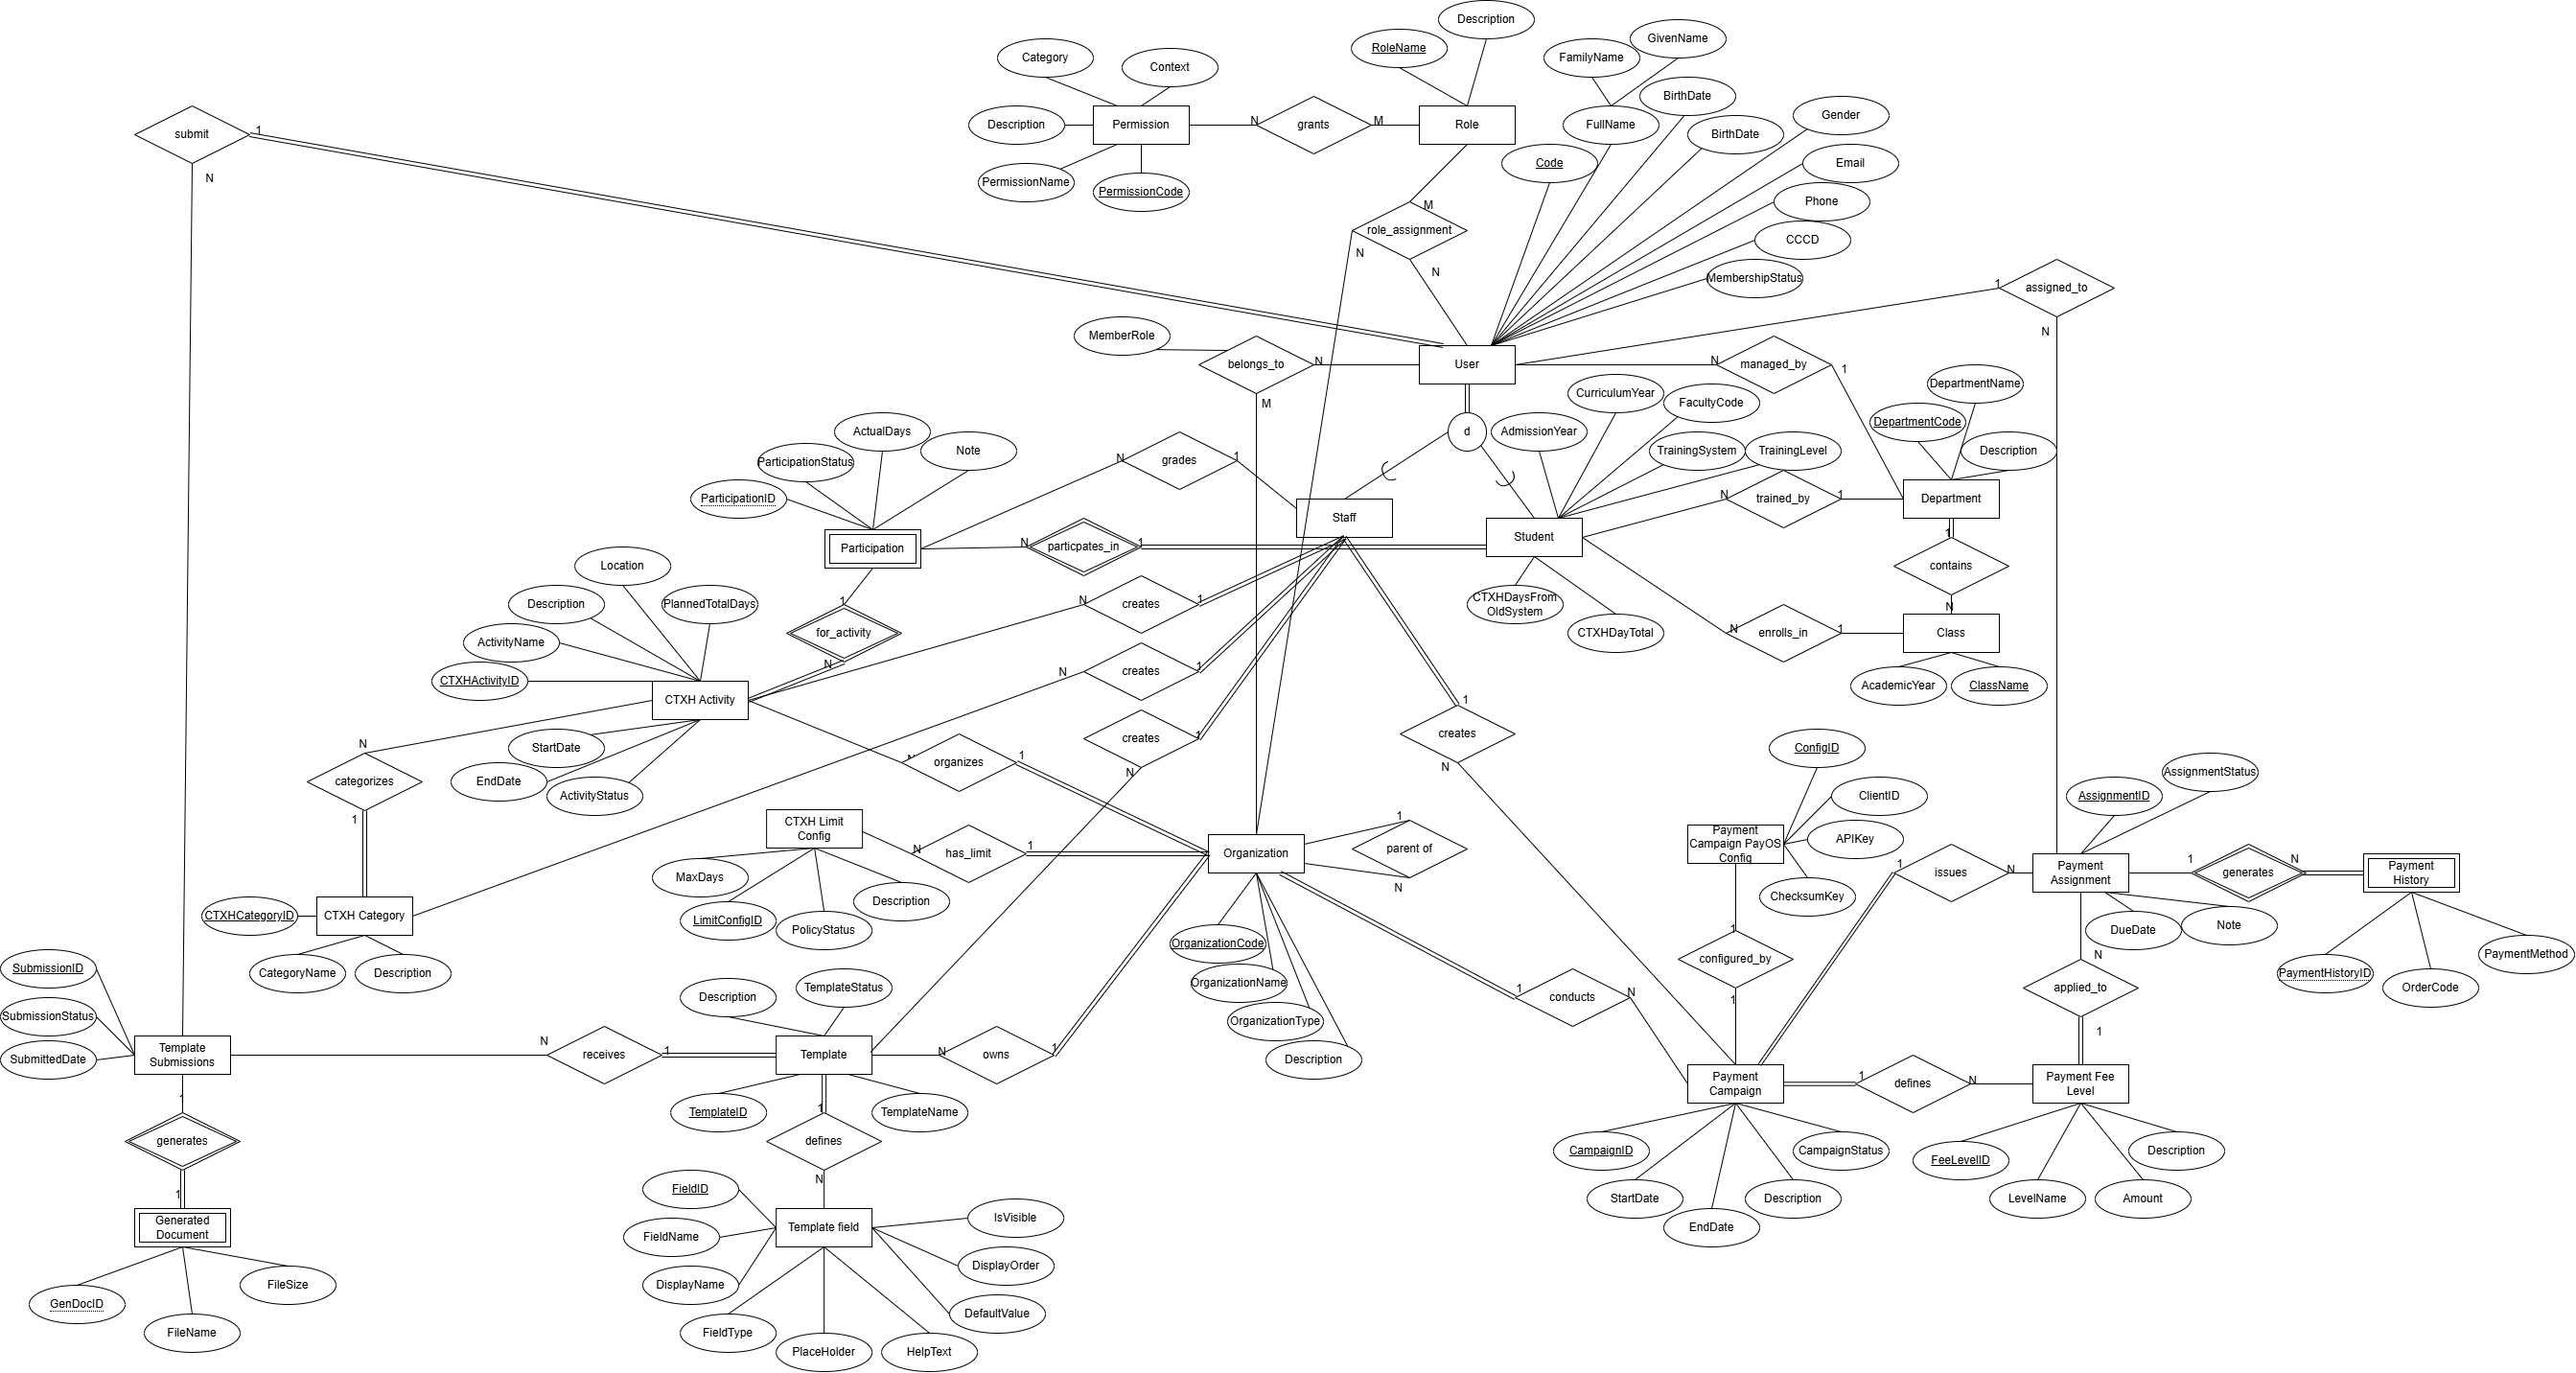
\includegraphics[width=1.0\linewidth]{Images/doanhoi_erd.drawio.png}
    \vspace{0.3em}
    \caption{Entity-Relationship Model cho toàn bộ hệ thống}
    \label{fig:doanhoi-erd}
\end{figure}

\begin{figure}[H]
    \centering
    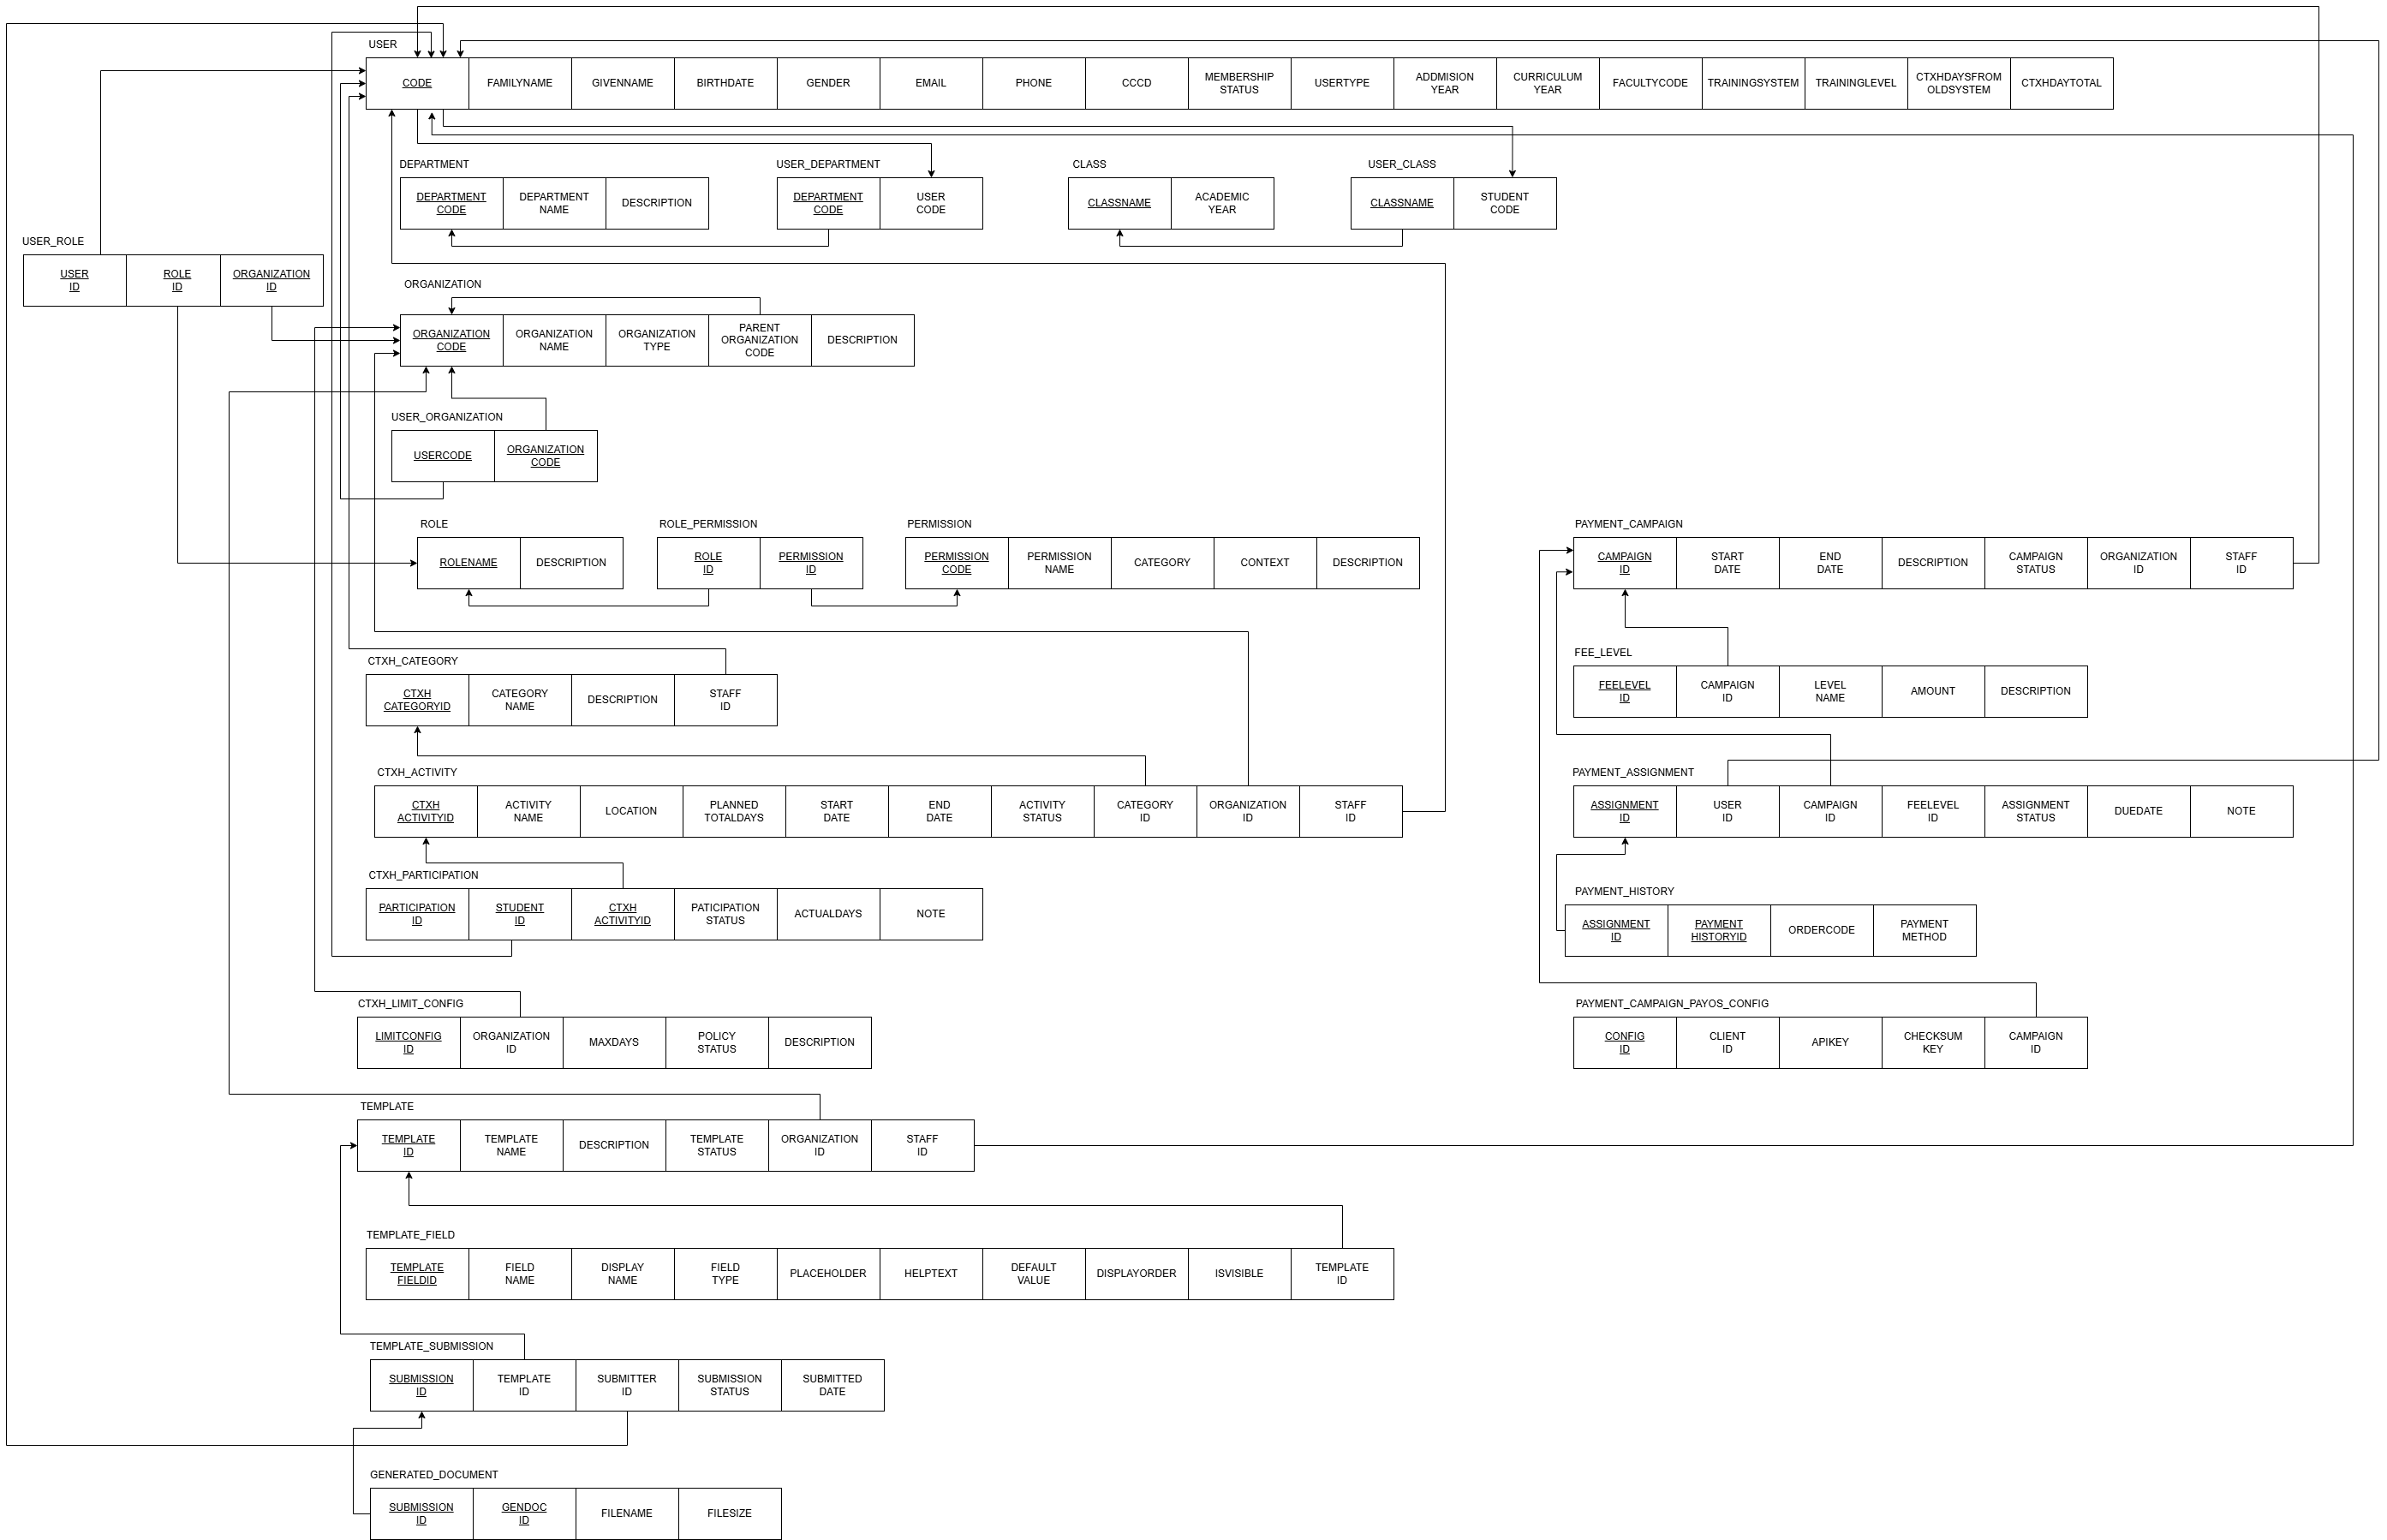
\includegraphics[width=1.0\linewidth]{Images/doanhoi_relational_db.drawio.png}
    \vspace{0.3em}
    \caption{Relational Data Model của toàn bộ hệ thống}
    \label{fig:doanhoi-relational}
\end{figure}

\subsubsection{Dữ liệu phục vụ Chatbot RAG}

\begin{table}[H]
\centering
\label{tab:ctxh_activity}
\begin{tabular}{|c|l|l|l|}
\hline
\textbf{STT} & \textbf{Thuộc tính} & \textbf{Kiểu dữ liệu} & \textbf{Mô tả} \\ \hline
1 & id & number & Mã định danh hoạt động CTXH \\ \hline
2 & name & string & Tên hoạt động \\ \hline
3 & description & string & Mô tả chi tiết hoạt động \\ \hline
4 & category.id & number & Mã danh mục hoạt động \\ \hline
5 & category.name & string & Tên danh mục hoạt động \\ \hline
6 & organization.id & string & Mã đơn vị tổ chức \\ \hline
7 & organization.name & string & Tên đơn vị tổ chức \\ \hline
8 & startDate & Date & Ngày bắt đầu hoạt động \\ \hline
9 & endDate & Date & Ngày kết thúc hoạt động \\ \hline
10 & totalDays & number & Tổng số ngày công tác xã hội \\ \hline
11 & location & string & Địa điểm tổ chức \\ \hline
12 & status & ActivityStatus & Trạng thái hoạt động (ACTIVE, UPCOMING, ...) \\ \hline
\end{tabular}
\caption{Cấu trúc dữ liệu CtxhActivity}
\end{table}

\textbf{Template văn bản chuẩn cho embedding:}

\begin{verbatim}
Tên hoạt động: [name], Mô tả: [description], Danh mục: [category.name], 
Tổ chức: [organization.name], Thời gian: Từ [start_date] đến [end_date], 
Ngày CTXH được cấp: [total_days] ngày, Địa điểm: [location]
\end{verbatim}

\textbf{Ví dụ cụ thể:} 

Tên hoạt động: CHIẾN DỊCH MÙA HÈ XANH CSE 2025, Mô tả: Năm nay, đội hình của khoa sẽ dừng chân tại mảnh đất Đồng Tháp xinh đẹp. Ở đây, chúng mình sẽ dành một tháng sinh hoạt cùng nhau, đồng thời cùng bà con cải thiện chất lượng cuộc sống tại địa phương, Danh mục: Mùa hè xanh, Tổ chức: Đoàn Khoa Khoa học và Kỹ thuật Máy tính, Thời gian: 7/2025, Ngày CTXH được cấp: 12 ngày, Địa điểm:  tỉnh Đồng Tháp